\documentclass[12pt]{scrartcl}

\usepackage[american]{babel}

\usepackage{graphicx}


\usepackage{paralist}
\usepackage{csquotes}
\usepackage[T1]{fontenc}
\usepackage{lmodern}

\usepackage[marginal]{footmisc}
\usepackage{hyperref}
\usepackage{pgfgantt}
\usepackage{float}
\usepackage[backend=biber,style=numeric-comp]{biblatex}
\usepackage{tikz}
\usepackage{xcolor}

% Colour Definitions
\definecolor{uniblue}{RGB}{000,032,091}
\definecolor{unigrey}{RGB}{199,201,199}
\definecolor{uniaccentblue}{RGB}{000,163,224}

\addbibresource{literature3.bib}

\usepackage{geometry}
% \geometry{a4paper,body={5.8in,9in}}
\geometry{a4paper}

\usepackage{amsmath, amsfonts, amssymb}
\usepackage{placeins}
\usepackage{subcaption}

\usepackage{setspace}

\setlength{\parindent}{0pt}

\renewcommand{\labelenumi}{\arabic{enumi}.} 
\renewcommand{\labelenumii}{\arabic{enumi}.\arabic{enumii}}
\renewcommand{\labelenumiii}{\arabic{enumi}.\arabic{enumii}.\arabic{enumii}}


\begin{document}

\title{Ranking of Classification Algorithms in AutoML}
\subtitle{A Comparison of Regression-Based Ranking and Preference Models
\\\vspace{2em}Bachelor's Thesis Proposal \& Work Plan}

\author{Helena Graf\\ 
\small{matriculation number: 7011643}\\ 
\small{hgraf@mail.upb.de}}
\date{\today}

\maketitle
\vspace{2em}

\begin{center}
\small{Supervisors:}\\
\large{Prof. Dr. Eyke H\"ullermeier}\\
\large{Prof. Dr. Axel-Cyrille Ngonga Ngomo}
\end{center}

\newpage


\section{Motivation}\label{sec:motivation}
%start with why ML is becoming more important
The potential of big data is evident, and an increasing amount of information is collected and available for analysis - but this potential is not utilized. In a white paper, the International Data Corporation claims that in 2012, out of the 2.8 zettabytes (ZB) of available data only 3\% were tagged as to enable further processing, and only 0.5\% were analyzed \cite{gantz2012the}. A follow-up paper in 2017 projects that in 2025, 15\% of the estimated 163ZB of global data will be tagged, and approximately 3\% analyzed \cite{gantz2017data}. While this is more optimistic, it still shows that there is a huge gap between the amount of data that could potentially be used and the amount of data actually available. This indicates that the demand of data to be analyzed cannot be covered by data scientists alone, and thus calls for automation of the process in a way that not much expertise in the field of machine learning is needed to gain insights about the collected data.\\

One of the most prominent machine learning tasks is classification: A class is assigned to an instance, for example clients of a bank may be either deemed creditworthy or not, based on factors like other existing credits or the job of the client. But selecting a fitting classifier for a new data set is difficult, since algorithm performances can vary substantially among data sets, and it is not feasible to simply apply a large number of them to empirically find a good match. For example, on a data set about the electricity prices in the Australian state New South Wales \cite{harris1999splice}, the predictive accuracy for the Multilayer Perceptron\footnote{With standart hyperparameters (L:0.3,M:0.2,N:500,V:0,S:0,E:20,H:a).} is 0.7887 \cite{cachada2017run3}. The predictive accuracy of the Random Forest\footnote{With standart hyperparameters (P:100,I:100,num-slots:1,K:0,M:1.0,V:0.001,S:1).} algorithm on the same data set is 0.9236 \cite{cachada2017run}, a much higher value. On a different data set, with the topic of vehicle silhouettes \cite{siebert1987vehicle}, we get a predictive accuracy of 0.7979 for the Multilayer Perceptron \cite{cachada2017run4}, and 0.7518 for Random Forests \cite{cachada2017run2}, showing an advantage of the former on this data set\footnote{Hyperparameters as above.}. So in each case, one would have picked a different algorithm in order to achieve the best results. In general, this means that for a different data set, a different algorithm might yield the best performance.\\
 
Since there is no one best classifier for all data sets, it is likely that how well a classifier performs on a given data set is dependent on properties of the data set, at least to some degree. Combined with the need for automated machine learning, this calls for an approach that considers past performances of classifiers for data sets in relation to properties of these data sets to automatically suggest well-performing classifiers for a new problem.

\section{Related Work}\label{sec:related_work}
The demand for aid in the process of selecting an algorithm has already led to the development of tools that automate machine-learning (AutoML). In the following paragraphs, three of such tools are outlined briefly.\\

Auto-WEKA is an AutoML tool that both selects a machine learning algorithm and optimizes its hyperparameters by using Bayesian optimization \cite{thornton2013auto}. It was first released in 2013 as an extension to the popular data mining software WEKA \cite{hall2009weka} to assist the large number of novice users of the software in selecting parameterized algorithms for their problems. The tool has since grown in popularity and is in version 2.0 as of March 2016 \cite{kotthoff2016auto}. In Auto-WEKA, the problem of selecting an algorithm and its hyperparameters is combined by treating the algorithm itself as a hyperparameter and searching the joint space of algorithms and hyperparameters for the best solution. An input data set is first preprocessed by means of feature selection. Then, Sequential Model-Based Optimization for General Algorithm Configuration (SMAC) is used to 'iterate[...] between fitting models and using them to make choices about which configurations to investigate' \cite{hutter2011sequential}. In the case of Auto-WEKA, this means that during the optimization process, a model is built, a configuration of hyperparameters that is promising regarding the current model and training data is tried out, and the result is fed back to the model. This cycle is then repeated until the allocated time has run out. Auto-WEKA exploits meta-knowledge, that is considering past performances of algorithms, to make decisions by always trying algorithms like Random Forests, which perform well on a large number of data sets, first. \\

% SK-learn
AUTO-SKLEARN has been described as a sister-package to Auto-WEKA and is an AutoML tool which is based on scikit-learn, a machine learning library for Python \cite{feurer2015efficient}. It works very similar to AutoML but extends it by adding a meta-learning pre-processing step to warmstart the Bayesian optimization and automatically constructing ensembles during optimization. During the pre-processing phase, performance values for the classifiers available in AUTO-SKLEARN are recorded on a set of data sets. For each data set, the algorithm which shows the best empirical performance is noted. Then, certain meta-features are calculated for each data set. The first step of the tool when given a new problem is to calculate meta-features of the data set. Then, the Manhattan distance to the other data sets is determined according to the meta-features, and the algorithms that are associated with the k-nearest data sets are used as a starting point for further optimization. The authors observe that the additional meta-learning and ensemble construction result in a more efficient and robust application. Their results show that meta-learning can be used to improve the overall AutoML process.\\

% ML-Plan
ML-Plan is an AutoML tool that instead of concentrating on hyperparameter optimization, aims to optimize the whole machine-learning pipeline \cite{wever2017automatic}. This is achieved by viewing machine-learning as a task, building a hierarchical task network out of those tasks, and then searching for a solution in the induced tree structure. In the tree, the root node contains the complex task of building a machine learning pipeline, inner nodes represent incomplete pipelines consisting of complex and possibly also primitive tasks, and leaf nodes are complete pipelines that include only primitive tasks. An example of this might be 'classify' as the root node, with an intermediate node on some level that contains the tasks 'build NN', 'train NN' and 'predict from NN'. The complex task 'build NN' would then further be decomposed, and could lead to a leaf node with n tasks 'Add layer', 'build NN' and 'predict from NN', which are all primitive tasks that do not need to be further decomposed. A best-first search algorithm in a modified variant is then used to find good solutions in this task network. While this variant does not use meta-learning in the process of optimizing the pipeline, the authors find that their results exceed those achieved by Auto-WEKA.\\

\begin{figure}
\tikzset{edge from parent/.style={draw,->}}
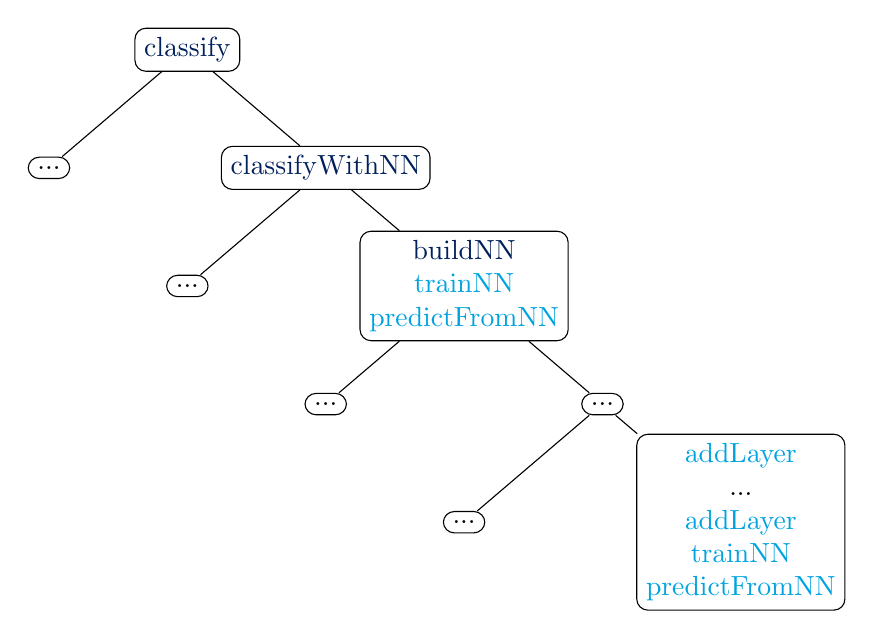
\begin{tikzpicture}[sibling distance=10em,
  every node/.style = {shape=rectangle, rounded corners,
    draw, align=center}]]
  \node {\textcolor{uniblue}{classify}}
    child { node {...} }
    child { node {\textcolor{uniblue}{classifyWithNN}}
    child { node {...} }
      child { node {\textcolor{uniblue}{buildNN} \\ \textcolor{uniaccentblue}{trainNN} \\ \textcolor{uniaccentblue}{predictFromNN}}
        child { node {...} }
        child { node {...} 
          child { node {...}  }
          child { node {\textcolor{uniaccentblue}{addLayer} \\ ... \\ \textcolor{uniaccentblue}{addLayer} \\ \textcolor{uniaccentblue}{trainNN} \\ \textcolor{uniaccentblue}{predictFromNN} } } } }
    };
\end{tikzpicture}
\caption{An example for how the complex task 'classify' might be broken down by ML-Plan. The figure is loosely adapted from \cite{wever2017automatic}. Nodes containing '...' represent an undefined amount of subtrees. \textcolor{uniblue}{Complex tasks} and \textcolor{uniaccentblue}{primitive tasks} are distinguished by their color.}
\label{fig:mltree}
\end{figure}


\section{Goals}\label{sec:goals}
The aim of this thesis is to test the assumption that given a new data set, one can derive an accuracy-based ranking of classification algorithms from their past performances by means of regression-based compared with preference-based ranking, and to compare the two methods. It is derived from the need for AutoML tools and the fact that related solutions so far have not exploited meta-learning in this way. If the hypothesis is true, this tool could be used as a pre-processing step in another Auto-ML framework similarly to how meta-learning is used in AUTO-SKLEARN, as a pre-processing step to speed up the whole process. The aim presented consists of multiple goals, which can be divided into required and optional goals.

\subsection{Required Goals}\label{subsec:required_goals}
Based on the general objective of the thesis, several goals should be achieved:

\begin{enumerate}
	\item Implementing a tool with the following functionality:
	\begin{enumerate}
		\item A pre-processing phase in which the performances of the available set of classifiers is calculated for a set of data sets, a regression model is fit to each of the classifiers, and a preference-ranker is fit to the ranks of the algorithms which can be deduced from their performance values.
		\item A method where the tool is given a data set and returns a ranking of classifiers for this data set.
		\item The possibility to choose between regression-based and preference-based ranking.
	\end{enumerate}
	\item Evaluate the predictions of both the regression and preference-ranking variant of the implementation by comparing them against each other, an oracle that represents the best ranking according to actual algorithms performances, and a best-algorithm baseline.
\end{enumerate}

\newpage
\subsection{Optional Goals}\label{subsec:optional_goals}
If the required goals have been met in less time than originally allocated, and the initial results are promising, addressing additional goals may be considered. The following list suggests possible optional goals. However, they may be replaced if while working on the thesis it becomes clear that more appropriate expansions exist.

\begin{enumerate}
	\item Adding automatic optimization of regression and ranking models with the help of ML-Plan and jPL\footnotemark{ } respectively \cite{intelligent2017jpl}.
	\item Extend the evaluation by comparing the tool with other AutoML solutions.
	\item Extend the evaluation by evaluating against a more intelligent baseline.
	\item Adding another layer to the search by including hyperparameters, possibly by means of iterative requests to the tool.
	\item Adding runtime and/ or complexity prediciton to allow for combined predictions.
\end{enumerate}
\footnotetext{A framework for the evaluation of preference learners.}

\section{Approach}\label{sec:approach}
As described in Chapter \ref{sec:goals}, the goal is to implement an AutoML tool that returns a ranking of classification algorithms for a given data set based on past performances of the classifiers by using regression and ranking models and evaluating the results. The implementation of this tool will be done in Java 8. Since the aim is to ensure a basic functionality, preliminary algorithms are going to be used both for regression and ranking models.\\ 

The first step therefore is to implement the pre-processing phase, which consist of computing the performances of classifiers on data sets. For the implementation of the classifiers, WEKA 3.8.1 is going to be used, which dictates the set of classifiers that will be included\footnotemark. The data sets will be fetched from OpenML.org, an open-source project where users can contribute data sets, implementations for machine learning algorithms, and algorithm runs. Since the results of the runs are available publicly on the website, some of the required data may be extracted instead of computed. OpenML.org provides the data sets in .ARFF format, and supplies a WEKA plug-in, which should ensure that these libraries work together smoothly. \\

\footnotetext{Meta-classifiers and ensemble-classifiers will not be supported.}

The next step is to add the functionality to fit preliminary regression models and a preference ranker to the performance data, based on properties of the data sets. This step also includes providing a method that can be given a data set and returns a ranking, based on the choice of ranking method either based on regression or a preference model. This method first needs to compute properties of the new data set. Then, for regression, it is going to use the preliminary regression model of each algorithm to get a predicted performance of each classifier for the new data set. These predictions are turned into a ranking. For the ranking model, the computed properties of the new data set can be fed to the model directly.\\

For the evaluation, it is necessary to generate a baseline and an oracle. Both can be obtained from the data of the pre-processing phase. Due to all performances of classifiers being recorded on all data sets, one can obtain an optimal ranking of classifiers for each data set from that same table. The baseline which is going to be used is counting the number of data sets for which a classifier is the best option, and then ranking them from overall best performance (best choice for most data sets) to worst. This can be obtained from the table of the pre-processing phase as well. The rankings of the oracle, the baseline, and the results of the tool are then going to be compared using the Kendall rank correlation coefficient.

\newpage
\section{Preliminary Document Structure}\label{sec:doc-structure}
The following structure will serve as an orientation during the writing process. While the chapters should remain the same, subsections may be added, removed or moved.

\begin{enumerate}
	\item Introduction
	\item Fundamentals
	\begin{enumerate}
		\item Meta-Learning
		\item Kendall Rank Correlation Coefficient
		\item JPL
		\item WEKA
	\end{enumerate}
	\item Approach
	\item Implementation
	\begin{enumerate} 
		\item Regression-based Ranking
		\begin{enumerate}
			\item Preliminary Regression Algorithm
			\item Automatic Algorithm Selection
		\end{enumerate}
		\item Preference Models
		\begin{enumerate}
			\item Preliminary Ranking Algorithm
			\item Automatic Algorithm Selection
		\end{enumerate}
	\end{enumerate}
	\item Evaluation
	\begin{enumerate}
		\item Computing the Accuracy of the Results
		\item Assessment of the Accuracy
	\end{enumerate}
	\item Related Work
		% Include RECIPE in final work also
		%Auto-WEKA
		%Auto-sklearn
		% ML-Plan
	\item Conclusion
	\item Literature
	\item Appendix
\end{enumerate}


\newpage
\section{Schedule}\label{sec:schedule}
The working time is going to be structured according to the schedule shown in Figure \ref{fig:schedule}. Variations due to unforeseeable circumstances may occur.

\begin{figure}[H]
% Gantt Chart of Schedule
\begin{ganttchart}[
%% Style Definitions %%
% Canvas %
x unit=0.6cm,
y unit chart = 0.65cm,
canvas/.append style={fill=none, draw=unigrey},
hgrid style/.style={draw=black!25, line width=.75pt},
vgrid={*1{draw=unigrey, line width=.75pt}},
title/.style={draw=none, fill=none},
% Title %
title label font=\bfseries,
title label node/.append style={below=0pt},
include title in canvas=false,
% Bar %
bar height=.5,
bar label node/.append style={align=left,text width=14em},
bar/.append style={draw=none, fill=uniblue},
% Group %
group height=.2,
   group peaks tip position=0,
group label node/.append style={align=left,text width=15em},
group/.append style={fill=black,opacity=0}
]{1}{16}

%% Chart %%
% Title %
\gantttitle[title label node/.append style={below left=0pt and -7pt}]{WEEK:\quad1}{1}
\gantttitlelist{2,...,16}{1} \\

% Elements %
\ganttgroup[]{Implementation}{1}{10} \\
\ganttbar{Phase 1}{1}{2} \\
\ganttbar[]{Phase 2}{3}{4} \\
\ganttbar[]{Evaluation}{6}{7} \\
\ganttbar[bar/.append style={fill=unigrey}]{Buffer}{5}{5} \\

\ganttgroup[]{Writing\footnotemark}{1}{13} \\
\ganttbar[]{Related \& Fundamentals}{1}{3} \\
\ganttbar[]{Approach \& Implementation}{4}{7} \\
\ganttbar[]{Evaluation \& Conclusion}{8}{10} \\
\ganttbar[bar/.append style={fill=unigrey}]{Buffer, Proofreading}{11}{13} \\
\ganttbar[]{Corrections}{14}{15} \\

\ganttgroup[]{Other}{5}{16} \\
\ganttbar[]{Presentation Preparation}{15}{16} \\

\end{ganttchart}

\caption{Sketch of the Work Schedule for the thesis.}
\label{fig:schedule}
\end{figure}

\footnotetext{The chapter 'Introduction' is not included since it will be written in parallel to other chapters, in small bits according to the progress of the thesis.}


\newpage
\printbibliography

\newpage
% Signatures and Delcaration %
Hereby supervisor and student confirm that this proposal is the basis for the topic assignment of the described work. The timetable and topic description are accepted by both sides as laid out in this proposal.

\vspace{6cm}

\begin{center}
     \begin{tabular}{l p{0.1\textwidth} r}
       \cline{1-1} \cline{3-3}
       \begin{minipage}[t]{0.4\textwidth}
         \centering
         Supervisor\\(Prof. Dr. Eyke H\"ullermeier)
         \end{minipage}
&
         \begin{minipage}[t]{0.2\textwidth}
         \end{minipage}
&
         \begin{minipage}[t]{0.4\textwidth}
           \centering
           Student\\(Helena Graf)
         \end{minipage}
     \end{tabular}
\end{center}

\end{document}
